\chapter{Transport Injuries}
\label{applications-double_dismod}

A compartmental model is not appropriate for all conditions.  Transport injuries have a wide range of outcomes, ranging from minor scratches to severe brain trauma to death.  Given some suffer acute injury while others sustain chronic conditions, traffic injuries violate the model assumption of a constant mortality hazard.  To address this disparity in mortality risk, transport injuries can be divided into short term and long term outcomes.  This method is also necessary for other injuries and diseases such as heart attack and stroke.

In the GBD 2010 Study, injuries are defined as all conditions codable to the ICD-9 and ICD-10 injuries chapter.  Transport injuries includes all road injuries for pedestrian, bicyclist, motorized two-wheeler rider, occupant in a motorized vehicle with 3 or more wheels, other road-transport injury and unintentional other transport injury.



Data only includes cases warranting hospital care and cases warranting treatment by health care professional but not hospitalization (other health care).

sources are verbal autopsy, surveillance systems, survey/census, police reports for mortality data yield cause-specific mortality rates and incidence



Only incidence data and finding prevalence data


DisMod:
hospital records -> incidence data for cause of injury incidence
discharge databases -> proportion cases for nature of incidence -> incidence for nature of injury
all short-term incidence -> short-term prevalence by cause or injury
portion of long-term incidence -> nature of injury prevalence





    \begin{figure}[h]
        \begin{center}
            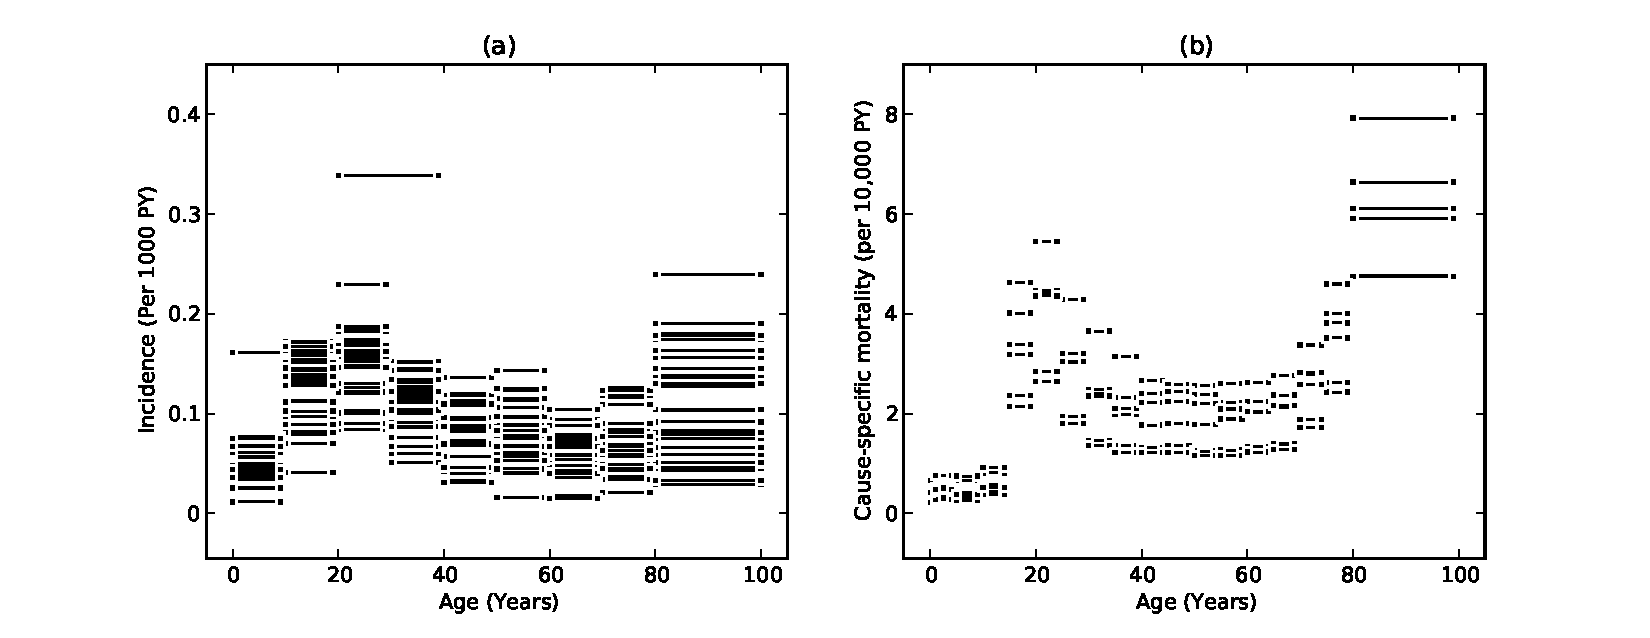
\includegraphics[width=\textwidth]{injury-traffic_data.pdf}
            \caption{Hospital and survey data for road injury and unintentional other transport injury for males in the region of North America, High Income.  Systematic review yielded only incidence (a) and the product of prevalence and excess mortality (b) data.}
            \label{fig:app-injury traffic data}
        \end{center}
    \end{figure}

    \begin{figure}[h]
        \begin{center}
            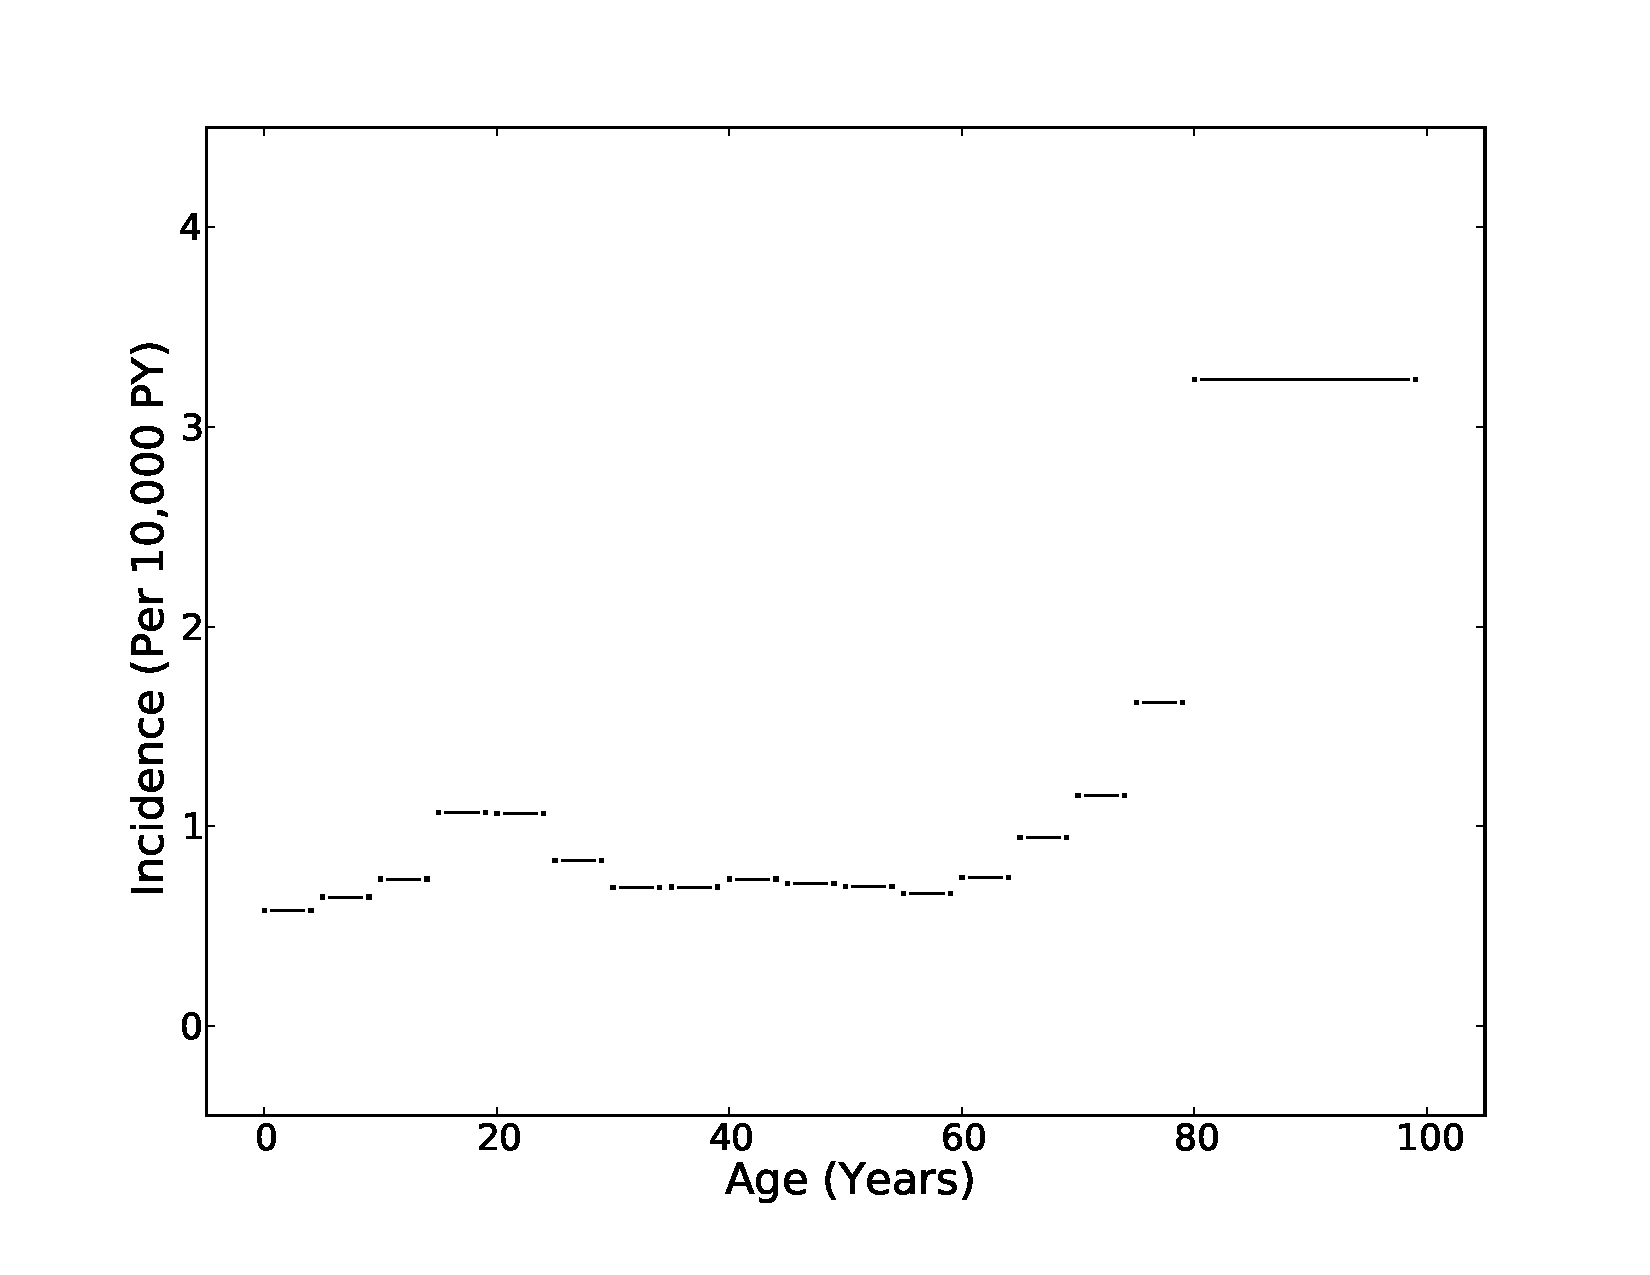
\includegraphics[width=\textwidth]{injury-brain_data.pdf}
            \caption{Long-term incidence data for moderate and severe traumatic brain injury in the region of North America, High Income.}
            \label{fig:app-injury brain data}
        \end{center}
    \end{figure}

Incidence data for moderate or severe traumatic brain injury warranting hospital admission or other health care in North America .

As discussed in Chapter 1.5, epidemiologic parameters, such as incidence, prevalence, remission, and with-condition mortality, are related by a logical requirement of internal consistency.  A prevalent case can only exist if there was a past incidence event and the current number of prevalence cases can be determined from past prevalent cases, new incident cases, deaths and remissions.  Modeling the parameters simultaneously produces a best estimate and plausible uncertainty bounds for incidence and prevalence that are internally consistent estimates for a single time, place and sex.


Moderate or severe traumatic brain injury sequelae SS183 SS212
SS183-Moderate long-term consequences of traumatic brain injury (with or without treatment)
SS212- Severe traumatic brain injury (short term) (with or without treatment)

